% Drawing 141/01-11 -- folder 141, batch 01, archive page 11 (PDF page 12).
% Transcription: en haut à droite, un triangle hachuré de traits verticaux, de sommets $0$ (en bas à gauche), $\infty$ (en haut) et $1$ (à droite).
% Kind: hatched triangle with vertices 0, 1, infinity. Method 2 (schematic redraw from the facsimile). Status: ok.
% Notes: As on the page: the triangle with heavy sides, its vertices labelled 0 (lower left), infinity (top) and 1 (right), and vertical hatching strokes, each drawn from a side to the base (computed on the sides). His strokes are seven or eight, unevenly spaced; seven are drawn. Redrawn 2026-11-12 (issue 128): to check again.
% Coordinates: 1 unit = 0.45 mm = 1/100 of the crop width (bbox in page fractions: [0.59, 0.1, 0.72, 0.18]).
% Redrawn by Claude (claude-fable-5-2), issue #128, 2026-11-12; not checked by a human; not compiled (no TeX in the session).
% Rights: reproduces part of the work -- behind RENDER_TRANSCRIPTS, never published by itself.
\documentclass[tikz,border=3pt]{standalone}
\usepackage{amsmath,amssymb}
\usetikzlibrary{patterns,arrows.meta}
\tikzset{pencil/.style={black!45}, struck/.style={black!35}, mpt/.style={circle,draw,inner sep=1.3pt}, pt/.style={circle,fill,inner sep=0.9pt}, opt/.style={circle,draw,fill=white,inner sep=1.1pt}}
\begin{document}
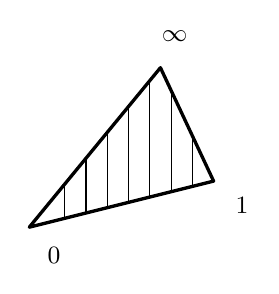
\begin{tikzpicture}[x=0.45mm,y=0.45mm,line cap=round,line join=round,font=\scriptsize]
\draw[very thick] (20,-73) -- (57,-28) -- (72,-60) -- cycle;
\draw (30,-60.8) -- (30,-70.5);
\draw (36,-53.5) -- (36,-69);
\draw (42,-46.2) -- (42,-67.5);
\draw (48,-39) -- (48,-66);
\draw (54,-31.6) -- (54,-64.5);
\draw (60,-34.4) -- (60,-63);
\draw (66,-47.2) -- (66,-61.5);
\node[inner sep=1pt] at (61,-19) {\small $\infty$};
\node[inner sep=1pt] at (27,-81) {\small $0$};
\node[inner sep=1pt] at (80,-67) {\small $1$};
\end{tikzpicture}
\end{document}
